%%%%%%%%%%%%%%%%%%%%%%%%%%%%%%%%%%%%%%%%%%%%%%%%%%%%%%%%%%%%%%%%%%%%%%%%%%%%%%%
%
% results
% Copyright (c) 2010 by tilo.mueller@rwth-aachen.de
% 
%%%%%%%%%%%%%%%%%%%%%%%%%%%%%%%%%%%%%%%%%%%%%%%%%%%%%%%%%%%%%%%%%%%%%%%%%%%%%%%

\chapter{Ergebnisse}

TODO: Roadmap (erst am Ende, "Kapitel 4 unterteilt sich in ... Unterkapitel und ...)

\section{Demographie}
Die Studiendurchführung ergab 1020 beantwortet Fragebögen. Nach bereinigung der Daten sind hieraus 856 vollständig bewertbare Fragebögen hervorgekommen.
Von den 856 Teilnehmern waren 204 (23,8\%) weiblich, 613 (71,6\%) männlich und 39 haben keine Angabe zu ihrem Geschlecht abgegeben. Die hohe Anzahl an männlichen Teilnehmern liegt vermutlich daran, dass die Umfrage über den Email-Verteiler der Technischen Fakultät der Universität Erlangen-Nürnberg verteilt wurde, welche einen höheren Männer- als Frauenanteil hat.
Im Mittelwert waren die Teilnehner 25,0 Jahre alt, mit einer Standardabweichung von 9,2 Jahren.
Interessant ist, dass trotz des niedrigen Wertes und der geringen Standardabweichung dennoch einige Fragebögen im Altersbereich von 45 bis 77 liegen. Dies wir in der weiteren Ausarbeitung gesondert betrachtet - denn selbst wenn ihre Anzahl nicht für statistisch exakte Aussagen reicht könnten hier dennoch interessante Ergebnisse gefunden werden.
Beim höchsten erreichten Bildungsabschluss zeigt sich dass ein Großteil der Teilnehmer entweder gerade studiert oder bereits einen Abschluss im Studium erreicht hat. Abitur und Bachelor/Master/Diplom zusammen geben über 90\% der Teilnehmer ab. Nur knapp über 5,7\% der Befragten hatten einen Haupt- oder Realschulabschluss.
Somit spiegelt die demographische Verteilung der Studienteilnehmer nicht die Gesamtzahl der Google-Nutzer in Deutschland wieder, da schon 2001 17,9\% der Deutschen mit Volks-/Hauptschulabschluss das Internet genutzt haben (nach Grafik "Nutzeranteil nach Bevölkerungsgruppen" \cite{ard2001internetusage}). In einer zukünftigen Arbeit zu diesem Thema sollten eventuell speziell die Gruppen "Kein Abschluss", "Hauptschulabschluss" und "Realschulabschluss" betrachtet werden.
TODO: 3-spaltige Tabelle mit allen Daten (Daten, relative Angaben, absolute Angaben)
\begin{figure}[H]
\centering
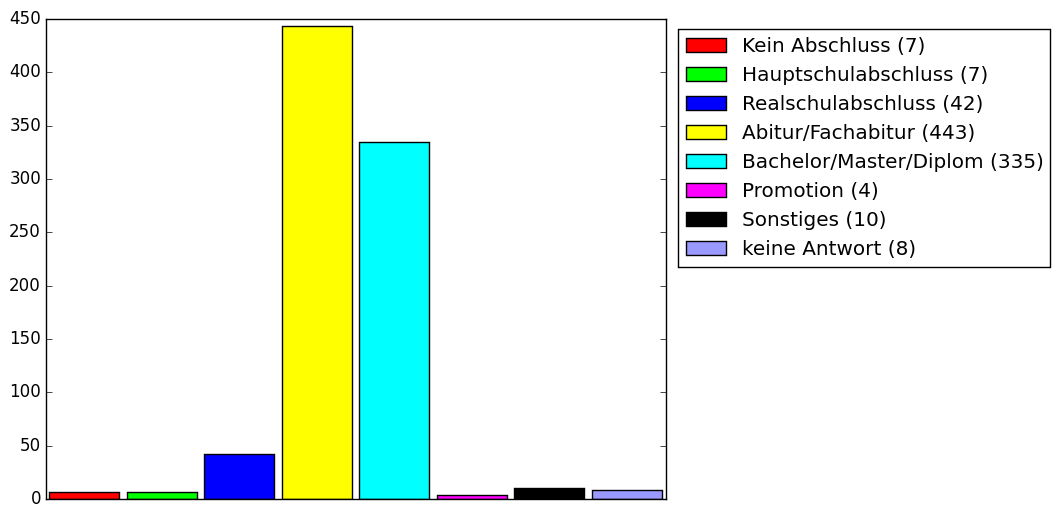
\includegraphics[scale=0.55]{images/schulabschluss}\\
\caption{Höchster Schulabschluss}\label{schulabschluss}
\end{figure}
Auch die Auswertungen zu der derzeitigen Arbeitsbeschäftigung zeigen ein ähnliches Bild - 77,0\% der Teilnehmer (659) waren zum Zeitpunkt der Studiendurchführung Studenten. Dahingegen sind nur 2,0\% in Ausbildung und 15,0\% berufstätig.
Das arithmetische Mittel der selbst eingeschätzten Informatikkenntnisse liegt auf einer Skala von 1 (keine) bis 5 (sehr hohe) bei 3,3. Hier wurde angenommen, dass im Durchschnitt ein Wert von 3,0 erreicht wird, da dies der Mittelwert der auszuwählenden Optionen war und man bei spezialisiertem Wissen von einer homogenen Verteilung ausgehen kann. Dass dieser Wert sehr nah an dem zu erwartenden Mittelwert von 3,0 liegt deutet darauf hin, dass die Umfrage trotz der geringen Anzahl an Realschülern und Hauptschülern dennoch Relevanz hat, wenn man weiterhin annimmt, dass der Wissenstand im Bereich Informatik hier der ausschlaggebende Faktor ist und nicht der Bildungsstand. TODO: In Grafik: Der größte Anteil hat mit 31,4\% einen Wert von 3 angegeben, kurz darauf folgen Kenntnisse von 4 mit 28,2\% und von 2 mit 24,2\%. Ein größerer Unterschied von über 10\% liegt zwischen denen die den höchsten Wert wählten (13,5\%) und denen die den niedrigsten Wert wählten (2,7\%).
Diese Statistik verschiebt sich stark, wenn man die Frage nach den Kenntnissen in der IT-Sicherheit betrachtet. Hier liegt das arithmetische Mittel bei 2,6, was um 0,6 niedriger ist als das arithmetische Mittel der IT Kenntnisse. TODO: Grafik oder Tabelle: Hier liegt das Maximum mit 30,9\% bei einem Wert von 2, Antwortmöglichkeit 3 und 1 haben 29,8\% respektive 16,8\%. Der Unterschied zwischen der Anzahl der Teilnehmer die mit 1 geantwortet haben und denen die mit 5 geantwortet haben liegt aber auch hier mit 12,1\% nicht sehr weit von dem Abstand aus der letzten Frage weg.
TODO: Korellation - Kein Bildungsabschluss in der Informatik bedeuted geringeres Wissen in IT Security: 77,5\% der Teilnehmer haben keinen Bildungsabschluss in der Informatik oder einem anderen IT-nahem Fachbereich.
Grafisch darstellen: steigende Funktion (Excel Tabelle, Pivottabelle, Youtube, Berechnung signifikant)

\section{Hypothesen}

Schon aus den ersten Fragen der Umfrage wird ersichtlich dass Google Dienste sehr aktiv genutzt werden. Auf "Wie aktiv nutzen Sie die folgenden Dienste? Google Suche:" antworteten fast 90% mit 4 und 5, davon sind 73,7% bei der 5 angesiedelt. Auch nutzen über die Hälfte der Umfrageteilnehmer (58,9%) Android mit einer Aktivität von 4 oder 5.

\section{Forschungsfragen}

\section{Sonstiges}
